Načrtněte grafy následujících funkcí:

\begin{enumerate}

	\item  $f(x) = ||||x| - 1| - 1| - 1|$

	\item  $f(x) = |\sin(x + \frac{\pi}{2})| + 1$

	\item  $f(x) = |\log_3|x+1|| - 1$
		\solution{
			Viz Obrázek~\ref{fig:grafy_funkci_c}.
			\begin{figure}[h]
				\centering
				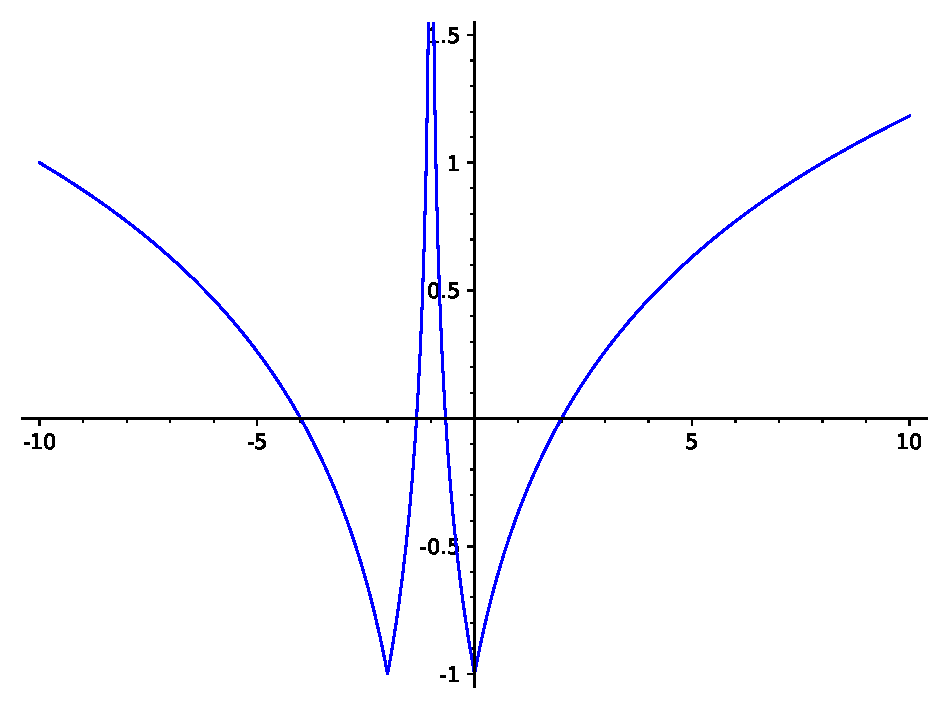
\includegraphics{cviceni_1/fig/c.pdf}
				\caption{$f(x) = |\log_3|x+1|| - 1$}
				\label{fig:grafy_funkci_c}
			\end{figure}
		}

\end{enumerate}

% sagemath:
% g = Graphics()
% f = abs(log(abs(x+1), 3)) - 1
% g += plot(f, (x, -10, -1), ymax=1.5)
% g += plot(f, (x, -1, 10), ymax=1.5)
% g.save('c.pdf')

